\section{Internet Protocol Security - IPSec}
IPsec est un ensemble de protocole visant à sécuriser les données au niveau de la couche réseau. 
Il est composé de trois protocoles : AH (\textit{Authentication Header}), ESP (\textit{Encapsulating Security Payload}) et IKE (\textit{Internet Key Exchange}).
IKE est utilisé lors de la négociation des paramètres du tunnel VPN. 
Les deux autres protocoles fournissent la sécurité des données en les encapsulant au sein du tunnel VPN. 

\subsection{Les protocoles AH et ESP}
Le protocole AH permet uniquement l'authentification. 
L'authentification se fait à l'aide d'un algorithme MAC \footnote{Message Authentication Code} tel que MD5 ou SHA-1.
Cette algorithme prend en input des éléments de l'en-tête IP et calcule un IVC \footnote{Integrity Check Value}.
L'IVC est ajouté dans l'en-tête AH et ce dernier est ajouté au paquet IP.

Le protocole ESP permet l'authentification et le chiffrement des données.

Un schéma des paquets formés est disponible sur la Fig.\ref{fig:ipsecHead} p.\pageref{fig:ipsecHead}.

\begin{figure}
	\centering
	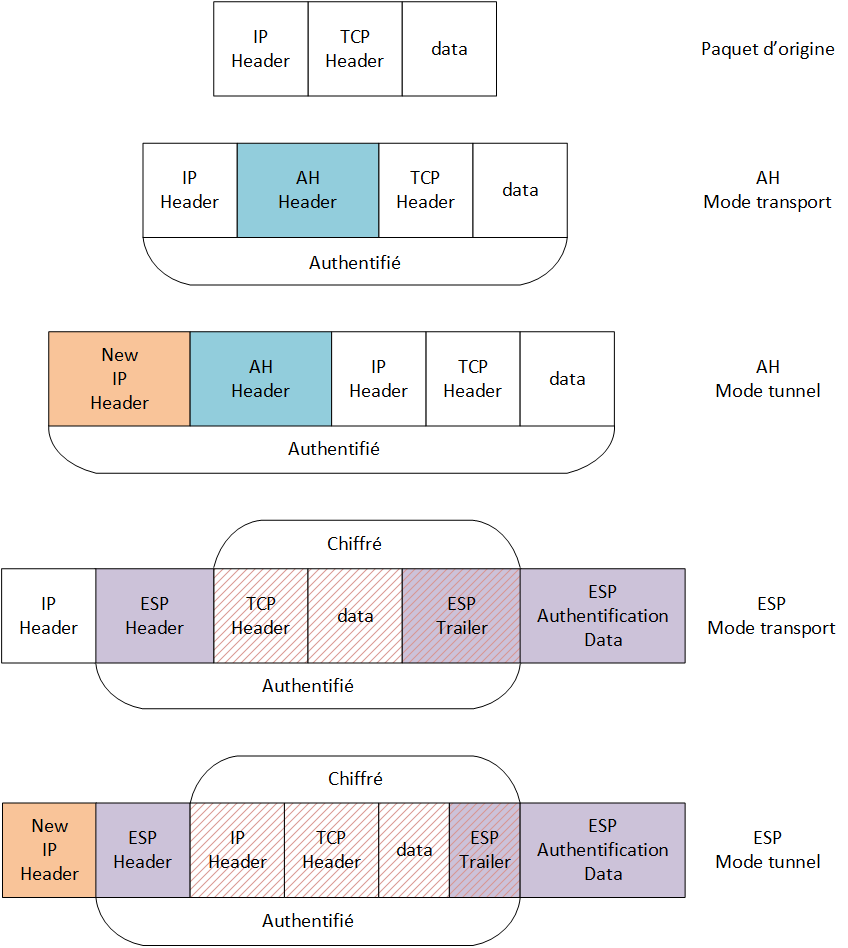
\includegraphics[width=16cm]{techno/IPSec-AH-ESP}
	\caption{Format des paquets IPSec}
	\label{fig:ipsecHead}
\end{figure}

\subsection{Les modes transport et tunnel}
Le mode transport est utilisé pour des connexions bouts-à-bouts entre deux hôtes.

Le mode tunnel est préféré lorsque l'un ou les deux hôtes de la communication sont des passerelles VPN.

\subsection{IPSec et le NAT}
Comme vu précédemment (Fig.\ref{fig:ipsecHead} p.\pageref{fig:ipsecHead}), IPSec protège les en-têtes des paquets IP.
Pour le protocole AH, le moindre changement au niveau des adresses IP provoque une erreur dans l'IVC vu que l'authentification s'applique au paquet entier.
Pour le protocole ESP, l'en-tête ESP est un paquet de la couche réseau. Il ne possède pas d'information sur les ports, qui sont des éléments de la couche transport.
Il n'est pas possible d'associer un port unique pour cette communication.

Pour palier à ces problèmes, une solution est d'encapsuler les paquets IPSec dans un autre paquet.
Ainsi le NAT-T (NAT-Traversal) encapsule les paquets IPSec dans un paquet UDP avec le port 4500 (par défaut).
Ainsi, c'est l'en-tête UDP qui sera modifier lors du transfert entre les deux hôtes et le paquet IPSec ne sera pas modifié.

\subsection{Security association}
Quand nous parlons de monter un tunnel, en réalité, nous synchronisons un état partagé entre les terminaisons du tunnel. 
Cet état partagé se nomme une SA (\textit{security association}) en IPSec. 
Une SA contient l'algorithme de chiffrement utilisé et les clés utilisées, l'algorithme d'authentification, un numéro d'identifiant, le \textit{security parameter index} (SPI), … 
Plus d'autres paramètres qui servent à maintenir les tunnels VPN. 
Les SA peuvent être créées manuellement ou gérées par l'IKE. 
Chaque terminaison possède deux SA, une pour le trafic entrant et une pour le trafic sortant. 
De plus, chaque paire est liée à un protocole. 
Les SA se caractérisent par un triplet formé du SPI, de l'adresse de destination et du protocole. 
Les SA sont stockées dans une SAD (\textit{security association database}). 
Cette SAD est utilisée pour déterminer quel protocole est utilisé pour les paquets sortants et pour fournir les paramètres pour déchiffrer et/ou authentifier les paquets entrants. 
Il est possible de combiner les SA pour créer des tunnels VPN complexe. 

Les SA sont des éléments simples, c'est-à-dire qu'elles traitent tous les paquets de la même manière. 
Pour un réglage plus fin, IPSec utilise des policies. 
Ces policies se basent sur les champs suivants des en-têtes du paquet.
\begin{itemize}
\item L'adresse de destination
\item L'adresse source
\item Le protocole de la couche transport
\item Le port source
\item Le port de destination
\end{itemize}
Elles servent à déterminer quels paquets à émettre sur quel tunnel, à dropper les paquets ne correspondant à aucune des règles décrites dans les policies. 
De la même manière que les SA, les policies sont stockées dans une SPD (\textit{security policy database}). 
Le fonctionnement est similaire, pour chaque paquet entrant ou sortant, le système consulte la SPD pour déterminer les règles à appliquer au paquet. Si une règle est trouvée, le système cherche après la SA correspondante.

\subsection{Le protocole IKE}
IKE a un seul objectif : procéder à des échanges de clé Diffie-Hellman pour sécuriser un tunnel VPN. 
Il négocie le chiffrement, l'authentification nécessaire au tunnel, qui satisfont les policies. 

IKE dérive du \textit{Internet Security Association and Key Management} Protocol (ISAKMP). 
ISAKMP est un framework qui fournit des outils pour la sécurisation des échanges et l'échange de clé. 
De plus, IKE utilise différents mode du protocole OAKLEY.
Il établit une SA en deux phases et il possède cinq modes d'échange, dont trois découlent d'ISAKMP.
Les deux derniers modes ne sont utilisés que lors de la phase deux.

\subsubsection{La phase 1 d'IKE}
La phase 1 crée un canal sécurisé entre les terminaux du tunnel pour déterminer les SA. 
Le canal sécurisé est créé après l'authentification des terminaux. 
Les SA de la phase 1 sont bidirectionnelles, c'est-à-dire qu'une SA sécurise le trafic entrant et sortant. 
Pour l'échange des SA de la phase 1, IKE possède deux modes d'échanges : 
\begin{itemize}
	\item Main mode
	\item Agressive mode
\end{itemize}

Le mode \textit{"main"} d'IKE travaille en trois étapes (voir Fig.\ref{fig:ipsmain} p.\pageref{fig:ipsmain}).
Il est utilisé lorsque les terminaux possèdent des adresses IP statiques. 
\begin{figure}[ht]
\centering
\begin{tikzpicture}
	\draw[-,ultra thick] (0,7) node [above] {Initiator} -- (0,0) ;
	\draw[-,ultra thick] (7,7) node [above] {Responder}-- (7,0);
	\draw[arrow] (0,6) -- (7,6) node [midway,above] {HDR - SA};
	\draw[arrow] (7,5) -- (0,5) node [midway,above] {HDR - SA};
	\draw[arrow] (0,4) -- (7,4) node [midway,above] {HDR - KE - NONCE$_i$};
	\draw[arrow] (7,3) -- (0,3) node [midway,above] {HDR - KE - NONCE$_r$};
	\draw[arrow] (0,2) -- (7,2) node [midway,above] {HDR - ID$_i$ - \textit{AUTH}};
	\draw[arrow] (7,1) -- (0,1) node [midway,above] {HDR - ID$_r$ - \textit{AUTH}};
\end{tikzpicture}
\caption{IPsec : mode "main"}
\label{fig:ipsmain}
\end{figure}
Premièrement, l'initiateur envoie un message contenant une liste des méthodes de sécurisation qu'il utilise. 
Le receveur choisit dans la liste reçue la méthode correspondant à ses policies et envoie sa décision à l'initiateur. 
Ensuite, ce dernier envoie sa clé privée pour créer le secret partagé de l'algorithme de Diffie-Hellman. 
Le receveur fait de même. Ils sont donc capables tous les deux de créer les clés. 
Les clés dépendent des méthodes d'authentification choisies. 
Finalement, l'initiateur envoie son identité et des informations sur l'authentification. 
Ces messages sont chiffrés et masquent donc l'identité des terminaux. 
L'échange se fait en six messages.

À la fin de ce mode, les terminaux sont d'accord sur les algorithmes de chiffrement et de confidentialité des données. 
Ils possèdent également les clés pour les algorithmes sélectionnés. 

Le mode \textit{"agressive"} fait le même travail de façon plus rapide, il n'utilise que trois messages (voir Fig.\ref{fig:ipsagg} p.\pageref{fig:ipsagg}).
Il est utilisé lorsque l'un des deux terminaux de la connexion possède une adresse IP dynamique.
\begin{figure}[ht]
\centering
\begin{tikzpicture}
	\draw[-,ultra thick] (0,4) node [above] {Initiator} -- (0,0) ;
	\draw[-,ultra thick] (8,4) node [above] {Responder}-- (8,0);
	\draw[arrow] (0,3) -- (8,3) node [midway,above] {HDR - SA - KE - NONCE$_i$ - ID$_i$};
	\draw[arrow] (8,2) -- (0,2) node [midway,above] {HDR - SA - KE - NONCE$_r$ - ID$_r$ - \textit{AUTH}};
	\draw[arrow] (0,1) -- (8,1) node [midway,above] {HDR - \textit{AUTH}};
\end{tikzpicture}
\caption{IPsec : mode "agressive"}
\label{fig:ipsagg}
\end{figure} 
Lors du premier envoi, l'initiateur émet la liste des méthodes de sécurisation, son identité et sa clé. 
Le receveur répond par son choix de sécurisation, sa clé, son identité et ses identifiants. 
Finalement l'initiateur s'authentifie auprès du receveur. 
Ce dernier message peut être chiffré.

Pour l'authentification d'un terminal, il existe trois méthodes : 
\begin{itemize}
	\item Kerberos
	\item Certificats	
	\item Public Key Infrastructure (PKI)
\end{itemize}

\paragraph{Kerberos}
Kerberos est un protocole réseau d'authentification par clé chiffré.
Il fournit une forte authentification à condition que tous les services utilisent Kerberos.
Il a été conçue par le MIT\footnote{Massachusetts Institute of Technology} à la fin des années 80.
Actuellement, il est recommandé d'utiliser la version 5, qui corrige des bugs critiques de la version 4.
Kerberos est disponible sur la plupart des systèmes d'exploitation actuels.
Une version gratuite est disponible sur le site du MIT, et il existe des versions commerciales.

Pour qu'un hôte puisse se connecter à un service, le système vérifie son identité, et le cas échéant accepte ou refuse la connexion.
Ce système repose sur deux serveurs sécurisés, un serveur d'authentification (AS\footnote{Authentication Server}) et un serveur d'octroi de ticket (TGS\footnote{Ticket-Granting Server}).
Ils forment dans la terminologie Kerberos un centre de distribution de ticket ou KDC\footnote{Key Distribution Center} en anglais.
De plus, Kerberos utilise des clés chiffrées pour toutes les communications.

\paragraph{Certificat}
Un certificat n'est rien de plus qu'une clé publique accompagnée d'un identifiant dont l'ensemble des informations sont signées par un tiers de confiance.
Ce tiers est ce que l'on appelle une autorité certificative (CA). 
Elle est reconnue au niveau mondiale.
Un utilisateur envoie sa clé publique au CA et reçoit en retour, après vérification, son certificat signé par la CA.

\paragraph{PKI}
Une PKI est un ensemble de composants et de processus informatiques, humains et techniques dont le but est de gérer la distribution et la vie des certificats.

\subsubsection{La phase 2 d'IKE}
Une fois la SA établie, les terminaux peuvent l'utiliser pour négocier les SA de phase 2. 
La phase 2 est un échange en Quick mode. 
L'échange se fait en trois messages. 
Lors de l'échange, il est possible de négocier plusieurs SA en même temps. 